\section{Cloud technologies}
Initially virualisation was thinked to solve a big problem: consolidate multiple apps on a single server. This because the "one application per sever" it's a waste of money and resources.
\subsection{Virtualisation}
\textbf{Computing virtualization} is a flexible way to share hardware resources (CPU, memory, storage ..) between different operating systems.
\begin{figure}
    \centering
    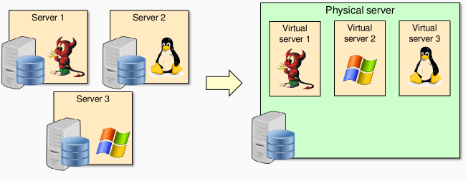
\includegraphics[scale=0.5]{images/virualisation.png}
    \caption{A virualization example}
    \label{fig:virt}
\end{figure}
So with virualization we use only one machine to run different OS and application (figure \ref{fig:virt}). The evolution of networking and the advent of optical fiber give the possibility to cloud computing to rise and became famous. 

Vitrualization has many pros:
\begin{itemize}
    \item \textbf{Isolation}
    \begin{itemize}
        \item Critical application could run in different and easily isolated OS
        \item Different services could run on the same hosts with an improved degree of isolation, we can assign a CPU core to one machine or isolate an application from the others to prevent issues caused by bugs or malicuious applications
    \end{itemize}
    \item \textbf{Consolidation}: Different OSes could transparently run on the same hardware at the same time saving hardware resources and money
    \item \textbf{Optimize energy consumption}: One machine running \textit{n} application use less electric energy than \textit{n} machines running one application
    \item \textbf{flexibility and agility}: Complete control over the execution information of all VMs, possibility to pause, resart, migrate and give more or less resources to the VMs
    \item \textbf{Possibility to duplicate a running VM}: For example to divide the traffic between two different machines
    \item \textbf{Disaster recovery}: Create snapshot and do rollbacks ecc.
    \item \textbf{Rapid deployment}: It's faster to deploy a VM instead of create a dedicated server for each service
\end{itemize}
Virtualization also brings with it limits and the challenge is try to handle it
\begin{itemize}
    \item \textbf{Additional overhead}: Each application has its own OS running (it use a lot of resources), however the overhead is usually considered acceptable for a wide range of different applications
    \item \textbf{More difficult to handle heterogeneous hardware}
\end{itemize}
There are tipically two scenarios of using the virtualisation technique, one is \textbf{Server virualisation} and the other is \textbf{Desktop Virtualisation} (like virtualbox), economicaly speaking server virtualisationis more important, desktop virtualisation is not a huge economic driver (most of this software is free). With virtualisation it's not important to have a physical machine with a given set of characteristics, we can create dynamically a virtual server with the requested characteristics. Users can buy tons of equivalent servers, with exactly the same hardware characteristics and aggregate them together in a datacenter and virtualize their resources.

Now let's see some definitions:
\begin{figure}
    \centering
    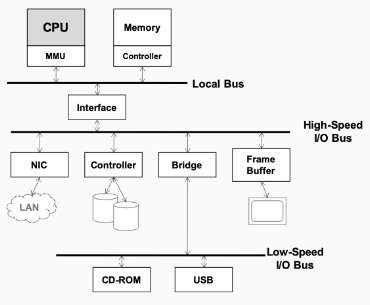
\includegraphics[scale=0.75]{images/computer architecture.png}
    \caption{Computer architecture}
    \label{fig:comparch}
\end{figure}
In figure \ref{fig:comparch} there explained the "normal" architecture schema of a computer, the goal of virtualisation is to \textbf{layer} all the things to create a modular like thing. Layering is a common approch to manage system complexity: it minimizes the interactions among the subsystems, simplifies the description of the subsystem. 

A layering model in computer system is the following:
\begin{itemize}
    \item Hardware
    \item Software
    \begin{itemize}
        \item Operating system
        \item Libraries
        \item Applications
    \end{itemize}
\end{itemize}
\begin{figure}
    \centering
    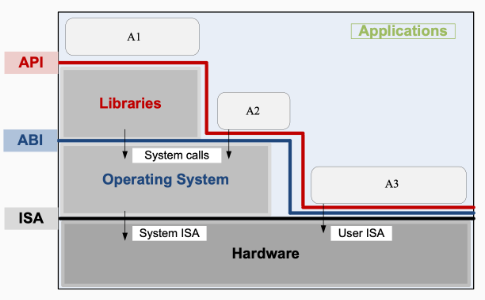
\includegraphics[scale=0.5]{images/layering.png}
    \caption{Layering schema}
    \label{fig:layers}
\end{figure}
As we see in figure \ref{fig:layers} an application use library functions (A1), makes system calls (A2), executes machine instructions (A3). This is possible because of three main interfaces (API, ABI, ISA)
\begin{itemize}
    \item \textbf{Instruction Set Architecture (ISA)}: Is at the boundary between hardware and software
    \item \textbf{Application Binary Interface (ABI)}: Allows application to access the hardware, it doesn't give privileged status but invokes system calls
    \item \textbf{Application Program Interface (API)}: Define the set of instructions the hardware was designed to execute and gives the application access to ISA
\end{itemize}
We spoke about \textbf{Virtual Machine} (VM) but what is it? A VM is a software emulation of a physical machine that executes OS and apps such as being in a physical one. The \textbf{Host OS} is the OS where the VM is running, is in charge of virtualise the hardware (it can include the Hypervisor). The \textbf{Guest OS} is the OS runned in the VM it doesn't know that is in a virtualised environment. The \textbf{Hypervisor} (or Virtual Machine Monitor) is the software in charge of the virtualisation process, it has to virtualise the resources. Virtualise means assigning a distinct set of resources to each VM and guaranteeing that each VM cannot get access outside its boundaries (in case resources cannot be partitioned arbitering the access to shared resources). So the Hypervisor manage virtualised hardware and system calls generated from Guest OS.

Computing virtualisation represent the most common approach for Cloud Computing according to IaaS model.


%-----------------------------------


\subsubsection{CPU Virtualisation}
We can ask the VMM to allocate many resources as many as we want and it will virtualize them.
The concept of virtualisation is different from the one of emulation:
\begin{itemize}
    \item[--] If the architecture of the virtual CPU is the same of the physical one, then the ISA (\textit{Instruction Set Architecture}) can be the same one (or a subset). We are in a case of \textbf{virtualisation}.
    \item[--] Otherwise if the virtual CPU's architecture is different from the physical one, then we talk about \textbf{emulation}. Emulation require the binary translation between the two ISAs and this is much slower.
\end{itemize}

We have alreay talked about VMs as \textbf{efficitent} (few overhead) and \textbf{isolated} (VMs don't step each other) copies of real machines.

We define the \textbf{Virtual Machine Monitor} (VMM) as a software that has to respect three charateristics:
\begin{itemize}
    \item It exports execution enviorments
    \item It executes some instrunctions on the real processor instead of on the virtual one.
    \item It should have complete control of the real system resources (but this not always happen)
\end{itemize}

There are three main different types of CPU virtualisation:
\begin{itemize}
    \item \textbf{Full virtualisation} where the guest OS can run unmodified. (ex VirtualBox).
    \item \textbf{Paravirtualisation} where the guest OS need to be modified in order to be executed
    \item \textbf{Hardware assisted Virtualisation} where the hypervisor exploit some hardware features (this method solved some issues from the other two solutions).
\end{itemize}

To isolate better the system we use a ring scheme. In x86 architectures there are often 4 rings that rapresent a privilage level. The kernel works in the ring 0 (most privileged level), instead applications in the ring 4 (less privileged).
Some modern OS uses just level 0 and 3 in order to reduce overhead and increase the CPU speed.
\begin{figure}[h]
    \centering
    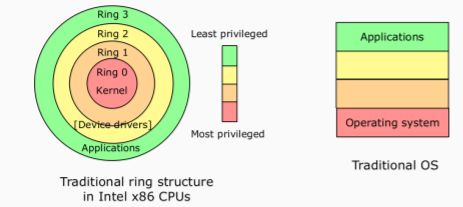
\includegraphics[scale=0.75]{images/rings.png}
    \caption{traditional ring structure of x86 Intel CPUs}
    \label{fig:ringstruct}
\end{figure}
When an application tries to run some instructions not available by the privilage level, the CPU handles them and execute a \textbf{TRAP command} that is a particolar INTERRUPT that move the execution to another ring (making a context switch).

Now the answer is where to put our guest OS.
There are two models:
\begin{itemize}
    \item The 0/1/3 (host, guest, application) model is problematic because the guest OS can run some instructions that it shouldn't and it can interfere with the VMM
    \item The 0/3/3 (host, guest, application) model solve the previous problem but is problematic because the guest OS is no longer protected from malicious applications that run over it.
\end{itemize}

There are two particular instructions that we have to menage in order to create a good isolation:
\begin{itemize}
    \item \textbf{Privileged instruction} are CPU instructions that generates TRAP routines if the CPU is running in the wrong context (For example using the system call HALT in ring 3, \textit{no privileges}).
    \item \textbf{Sensitive instructions} are CPU instructions that provide some information about the physical state of the processor (ex. its privileged level). If we want to virtualize a guest OS we want these instructions to be privileged.
\end{itemize}

We invoke \textbf{TRAP} routines when:
\begin{itemize}
    \item We try to execute instructions not allowed (Exceptions)
    \item System calls are invoked
    \item There are hardware INTERRUPTs.
\end{itemize}
In the OS there are memorized groups of instructions to be executed for every type of INTERUPTs (\textbf{Interrupt Description Tables}, IDT). In traditional way, when a TRAP routin is invoked, the CPU jumps to these tables (with a \textbf{IRET\footnote{This technique is very slow, it parse several memory location} instruction}) and execute indicated instructions in a privileged way. This is a context switch and it has a cost! The new way uses is more performing, it uses specific registers to store the routine and then calls SYSENTER and kernel runs in a very fast transition.

In an emulated environment the guest OS runs in an unprivileged environment (as an application). If it requires an instruction not allowed, the CPU launches a TRAP that the VMM intercepts. After that the VMM emulates the instruction and gives control back on the guest OS execution that will try to handle it. 
Thanks to this method the guest OS can execute some operations (like shutting down) because of the VMM emulation. So the guest OS keeps not knowing that is running over a VM.
\begin{figure}[H]
    \centering
    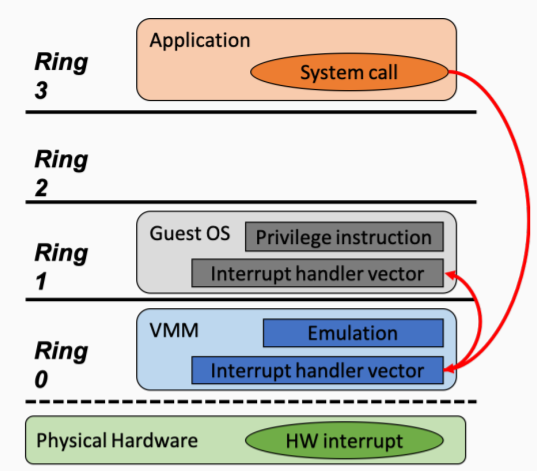
\includegraphics[scale=0.37]{images/trap in emulation.png}
    \caption{trap routine in emulated OS}
    %\label{fig:ringstruct}
\end{figure}
If the handle instruction needs to execute others privileged instructions (applications use library that provides functions) it will give control back to the VMM (invoking a new trap)
\begin{figure}[H]
    \centering
    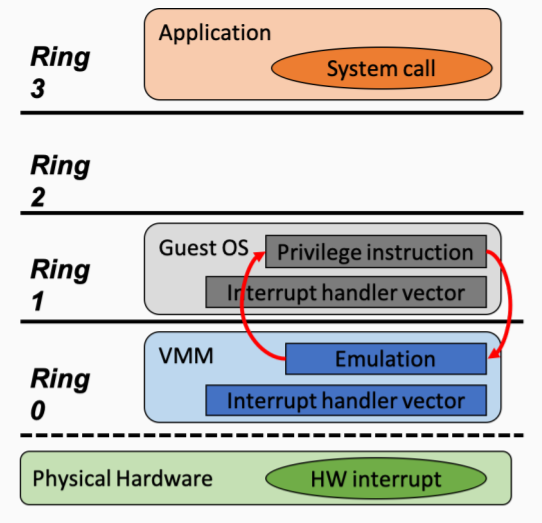
\includegraphics[scale=0.37]{images/trap in emulation (2).png}
    \caption{trap routine in emulated OS (2)}
    %\label{fig:ringstruct}
\end{figure}
If the TRAP is caused by an hardware INTERRUPT, CPU invoke the VMM interrupt handler; the VMM then will jump to the interrupt handler of guest OS.
\begin{figure}[H]
    \centering
    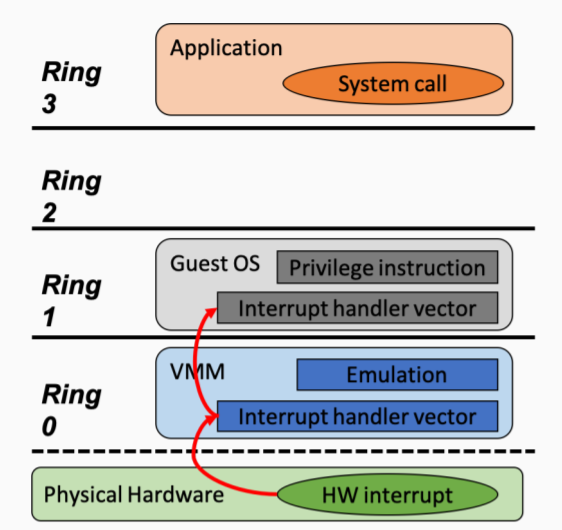
\includegraphics[scale=0.37]{images/trap in emulation (3).png}
    \caption{trap routine in emulated OS (3)}
    %\label{fig:ringstruct}
\end{figure}
The \textbf{trap and emulation} paradigm that we have just discussed has two problems:
\begin{itemize}
    \item It causes huge costs in terms of time-consuming; in fact the CPU has to switch between privilege levels many times for every TRAP invoked.
    \item Many architectures are not made to be virtualized. They have some sensitive instructions that don't trap if executed (so the VMM can't detect them).
\end{itemize}
Let's see some possible solutions:
\begin{itemize}
    \item Detect and interpret them dynamically (very long and slow process)
    \item Use \textbf{Dynamic Binary Translation} (DBT): this doesn't require any OS modifications or hardware supports. The VMM dynamically (at runtime) translate sensitivity instructions in instructions that trap. This causes hight overhead that can be reduced introducing caching techniques. \textbf{Vmware wokrstation} is a combination of Trap and Emulation paradigma and the DBT; it makes possible to push the guest OS to the ring 1 and the VMM to ring 0.
    \item Change the OS patching it (this is a long elaboration). This is called \textbf{Para-Virtualisation}: the guest OS is explicitly deprivileged (to ring 1) but is enriched with some mechanism to communicate with the hypervisor (particular hypervisor calls). This is a faster solution (it doesn't need to emulate stuff) but require OS modifications. It's not compatible with Windows OS.
    %\item Make all sensitive instructions privileged. 
    \item \textbf{Hardware-assisted virtualisation} (HVM). The idea is to have a hardware support that promote sensitive instructions as privileged or dynamically configure a trap mechanism (in the VMM). In particular CPU creates a new model of privilege levels (non-root mode) over the native one (root mode) and puts the guest OS on the lower level of non-root mode and on the ring 3 of root mode.
    \begin{figure}[H]
        \centering
        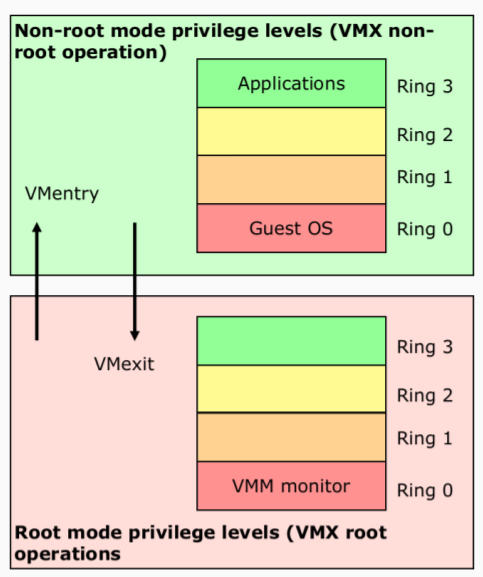
\includegraphics[scale=0.37]{images/HVM.png}
        \caption{HVM structure}
        %\label{fig:ringstruct}
    \end{figure}
    Through VMLAUNCH and VMRESUM instructions (VM exits) the CPU enters and exits from non-root and root mode in order to temporarily give the control to the VMM just to execute the privileged instruction (emulating the correct behavior). This solution introduce a great simplification: the time of trapping is reduced and the DBT method is avoided; Furthermore there's no OS modification.
    \begin{figure}[H]
        \centering
        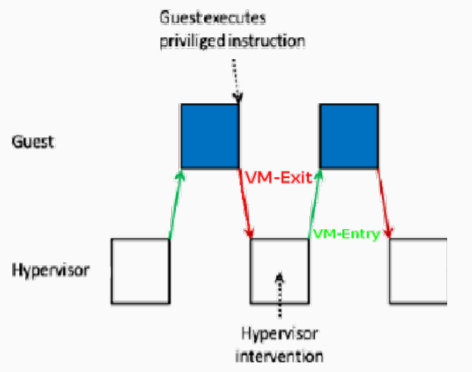
\includegraphics[scale=0.37]{images/VM exits.png}
        \caption{execution of privileged instructions in HVM}
        %\label{fig:ringstruct}
    \end{figure}
    The \textbf{Virtual Machine Control Structure} (VMCS) is a new element of memory that allows the switching between the two modes memorizing:
    \begin{itemize}
        \item Guest state (stored during VM exits and loaded during VM entry)
        \item Host Processor information
        \item Some control data
    \end{itemize}
    But there's still a problem: nested virtualisation is much slower because nested VMs can't use HVM.
\end{itemize}


\subsubsection{Memory virtualisation}
Modern Operating system use "memory paging" (the physical memory is interpreted into pages) to access as contiguous dispersed locations in the physical memory; the OS keeps a set of tables to translate the virtual memory address into physical ones (this operation is handled by \textbf{MMU}). Virtual addresses, used by processes (starting from 0), are translated by the MMU to physical addresses using big hash table for the mapping.

\begin{figure}[h!]
    \centering
    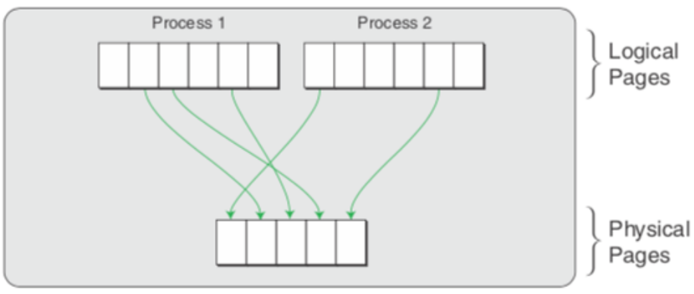
\includegraphics[scale=0.3]{images/mapping_mm.png}
    \caption{Mapping from LPNs to PPNs}
    \label{fig:mapping_mm}
\end{figure}

If we take a look at fig \ref{fig:mapping_mm} we see the walks that hardware does in order to determinate the corresponding physical address.

Another task of the MMU is to manage the \textbf{TLB} (\textit{Translation Lookaside Buffer}). This is a cache with very fast access that keep stored the association of recently used logical pages with  physical pages. When a process asks for a logical address the OS tries to find the association in this cache; if the result is missing than it will ask the MMU for it.

But why we would like to virtualize memory?
\begin{itemize}
    \item \textbf{Simplicity}: Every process gets illusion of whole address space (apps doesn't have to care about pages).
    \item \textbf{Isolation}: Every process is protected from every other.
    \item \textbf{Optimization}: The OS can optimize how pages are used; this reduces space requirements.
\end{itemize}

In VMs is required another level of translation (Guest virtual address $\rightarrow$ Guest physical address $\rightarrow$ Machine physical address). To avoid this step a "\textbf{Shadow Page Table}" is introduced: it stores and keeps track of the mapping between Guest logical address and Machine physical pages, it's invisible from the guest point of view and it'll be used by the CPU for a translation when the guest is active.

How it works:
\begin{itemize}
    \item The VMM maintains the association of physical pages and machine pages in internal data structures.
    \item The VMM stores associations of logical pages and machine pages inside shadow page table exposed to hardware.
    \item The TLB keeps stored most recently used logical pages and the correspondents machine pages.
\end{itemize}
\begin{figure}[h!]
    \centering
    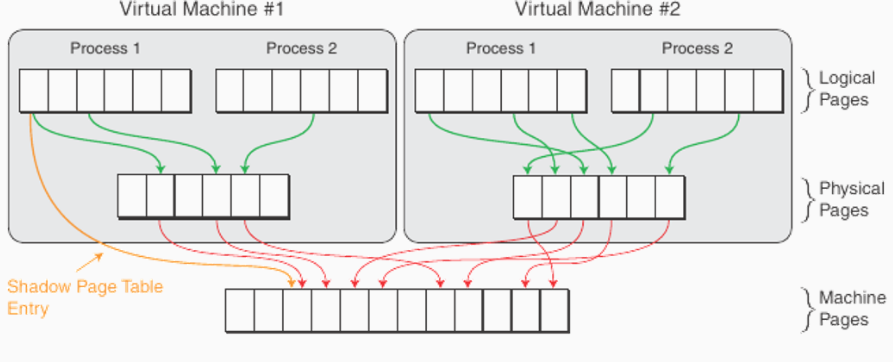
\includegraphics[scale=0.3]{images/mapping2_mm.png}
    \caption{CPU see only orange arrows, VMM see only red ones}
    \label{fig:mapping2_mm}
\end{figure}

The VMM is in charge of keeping the Shadow Page Table synchronized with the guest OS page table.
An important problem is the extra overhead that is introduced for keeping updated the Page Table when guest OS makes some updates in its ones. In order to avoid this overhead Intel and AMD have introduced two technologies (Extended Page Table and Rapid Virtualisation Indexing) that allow to do again a double translation: in fact traditional page tables translate logical pages into physical ones and the VMM maintains physical pages and machine pages mappings in an additional level of page tables, called \textbf{nested}.
\begin{itemize}
    \item Both the traditional page tables and the nested page tables are exposed to the CPU (now CPU know all the "path").
    \item Now there's no need to expose Shadow Page Tables, CPU does all the work (fig. \ref{fig:mapping3_mm})
\end{itemize}
\begin{figure}[h!]
    \centering
    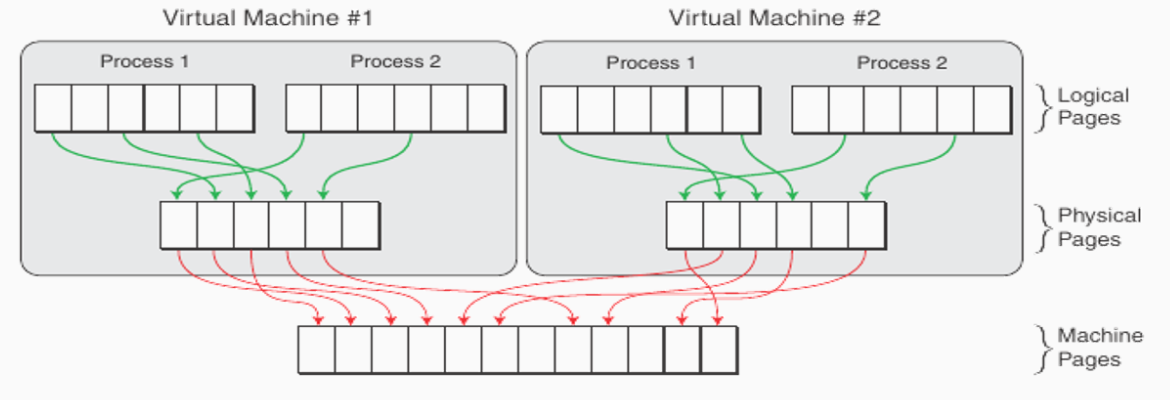
\includegraphics[scale=0.3]{images/mapping3_mm.png}
    \caption{Extended Page Table}
    \label{fig:mapping3_mm}
\end{figure}

This approach removes the need of VMExits (that involve context switches) associated with page table virtualisation. Guest could now keep update its page table without any overhead.

In addition to this now there's no need to use Shadow Page Table anymore; anyway this increases the cost of a single page walk; so now the TLB cache becomes critical to guarantee good performance (for example Intel processors uses two TLBs, one for normal pages and one for huge pages).

One last step to optimize memory virtualization technologies is to add an identifier for each virtual processor in order to allow several virtual processors coexist on the TLB at the same time (and don't leave the possibility to a processor to access to other processor caches).


\subsubsection{I/O virtualization}
As other resources, there are several techniques adopted for virtualizing I/O devices:
\begin{itemize}
    \item Device emulation
    \item Para-virtualized device
    \item Direct assignment
\end{itemize}
The choice of the technique depends on the type of device and if it Shared/Dedicated to a single Guest OS.

The problem with I/O devices is that every hardware manufacture does its devices as it wants. In order to make them working with every OS, they must provide \textbf{drivers\footnote{they standardise the method for the communication}}.

\myparagraph{Device emulation}
In \textbf{Device emulation} VMM proposes to the Guest OS an emulated device. The guest OS has no idea that is an emulated device (it just tries to do instructions that trap on the native OS) and the VMM has to remap device communication with the physical device in native OS (VMM has to emulate the response of the I/O for the Guest OS that doesn't care to the real drivers).
So the guest OS keeps using its drivers that are completely detached form the ones of native OS.

This approach is simple and easy to set up (and transparent to the guest OS): there's no need to install dedicated drivers and a single physical device could be multiplexed with several emulated device.
The disadvantage is that I/O operations are generally slower than physical ones and that could increase substantially the CPU load.

\myparagraph{Para-virtualization}
In \textbf{Para-virtualized device} guest OS is enriched with dedicated drivers (Guest OS knows that it's virtualized). It's very similar to CPU virtualization but in this case is simpler: it requires only to create new dedicated device drivers instead of modifying a kernel (making things easier and faster without having to fake anymore driver answers). In addition you need just a single para-virtualized driver for every device.
An example of usage of this method is realized by the Memory Ballooning driver. This is a special driver that stands besides traditional drivers and allow to communicate (directly to the VMM) how much memory is used in VM. This allows to make the memory allocation dynamic without over-committing.

\myparagraph{Direct assignment}
In \textbf{direct assignment} the VM communicate directly with physical I/O devices. In this case, the drivers used are the ones of the guest OS and not of the host OS.

\textbf{PCI-passtrough} is an example of application of this method. In particular it allows to use physical PCI devices (graphics card and network card) inside VMs.

Apparently the problem is always the same: how a device can write/read in the physical memory?
As we discussed above, the VMM perform some kind of translation (with relative overhead) from logical addresses to physical ones. \textbf{IOMMU} is an extension of the MMU that remaps addresses accessed by the hardware to the same table used to map guest-physical address to host-physical addresses.

Furthermore the PCI-e standard defines SR-IOV, a technology that allows to create a partition of the network interface card so that different parts can be assigned to different VMs.

In conclusion, direct assignment is the fastest and less expensive technique of I/O virtualization.


\subsection{Hypervisor architectures}
Traditionally there are two main kinds of architectures; a hybrid approach is sometimes used too.

\subsubsection{Type 1}
The hypervisor of type 1 runs directly on bare metal (hardware). On the top of it there are all guest VMs.
This is the type that guarantee best performances (because there is no OS in the middle) but that's quite complex in installation: in fact a hypervisor has less functionality of a real OS but needs to have the proper drivers for all hardware.
Most famous implementations are Vmware ESXi, Xen and Microsoft Hyper-V.

\subsubsection{Type 2}
The hypervisor of type 2 runs over a host OS as a common application. This is a less performing technique but easy to install and configure. Most famous implementations are VirtualBox and VMware workstation.

\subsubsection{hybrid type}
The hybrid hypervisor is implemented in the OS kernel (the host OS is the hypervisor itself). This technique allow very good performances.

\begin{figure}[h!]
    \centering
    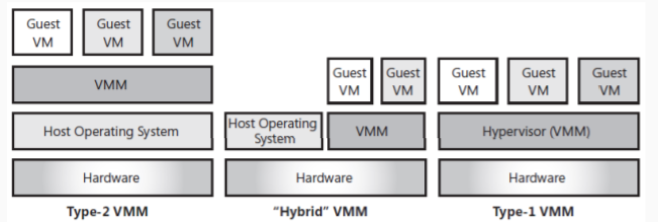
\includegraphics[scale=0.4]{images/VMM architectures.png}
    \caption{Graphical representation of VMM types}
    %\label{fig:mapping2_mm}
\end{figure}


\subsection{OS-level virtualisation}
Let's summarise VMs advantages:
\begin{itemize}
    \item they allow to run different OS on the same architecture
    \item they provide an isolated environment for single applications 
    \item excellent isolation with CPU and memory
\end{itemize}
and disadvantages:
\begin{itemize}
    \item Important overhead executing the guest OS (huge usage of CPU and memory)
    \item Necessity to constantly take care and keep updating hundreds of different OS
    \item more OS booting time
\end{itemize}

But do datacenters need to install multiple copies of same OS? It's more useful instead having a main OS (that's Linux) that share its kernel to different processes.
This is called \textbf{lightweight virtualisation}. In order to substitute VMs, it guarantees with less overhead:
\begin{itemize}
    \item scalability
    \item elasticity
    \item isolation
\end{itemize}

The idea is to run the OS virtualized without having a hypervisor (it's the Linux itself), replacing VMs with containers (virtual environments). Of course there are some limits compared to VMs but it's enough for lots of operations.

There are some requirements to implement lightweight virtualisation:
\begin{itemize}
    \item possibility to control resources (CPU cores, RAM) of physical machines among processes. In particular resources are dedicated to sets of processes.
    Working with groups of processes is better:
    \begin{itemize}
        \item you can menage and control them as a single class
        \item they are able to talk each other easily (for example inside the same application)
    \end{itemize}
    \item security and isolation (processes don't have to affect others). Isolation is so important for some reasons:
    \begin{itemize}
        \item a process must be always safely executed (with no possibility to compromise the entire machine), with some amounts of resources dedicated to.
        \item hardware isolation must be avoided; it will overkill all the technology.
    \end{itemize}
    \item possibility to menage an entire datacenter as a unique entity. This allows more portability
\end{itemize}

\subsubsection{Cgroups}
Linux kernel provides some primitives to limit, account (useful for billing), isolate and deny resources to processes or groups of processes.

Let's see main instructions:
\begin{itemize}
    \item \textit{cgcreate} create a cgroup
    \item \textit{cgset} set CPU.shares values to cgroups. They are relative values that make sense only with other values
    \item \textit{cgexec} execute the cgroup
\end{itemize}

Given two cgroups with 1024 and 512 CPU.shares, if the architecture has a single core, resources will be allocated with a proportion of 66\% and 33\%.
Instead if the architecture has multiple cores, resources will be allocated with a proportion of 100\% and 50\%.

\subsubsection{Namespaces}
\textbf{Namespaces} are virtual environments (highly related with cgroups) where processes visibility is limited to the partition itself (so two namespaces will have completely different IP addresses routine tabs, stacks, ...).

Currently there are seven different types of namespaces: IPC, Network, Mount, PID, User, UTS, Cgroup. Every type than can have multiple instances.
%DOMENICO UNO DI NOI\footnote{DOMENICO SIRACUSA CAPO DELLA TRAP PER FAVORE INGRAVIDACI} 

In Linux all processes are generated by a \textit{fork()} function invoking starting from the \textit{init()\footnote{nowadays called \textit{systemd}}} process. So processes generate other processes, creating a tree. A process with enough privileges and under some conditions can inspect another process by attaching a tracer to it or may kill/suspend it.

PID namespace enable multiple nested process tree (fig. \ref{fig:nestedtree}).
The main advantage of nested tree is that the first process of sub-tress will be seen as the "init" (PID 1) from its children (thanks to isolation).
The parent PID namespace know about all the processes; instead children ones don't know about the processes in the yellow area.
So a single process can now have multiple PIDs associated to depending from which which process/namesapce you are looking from. In particular the PID will be implemented as an array of values witch id/namespace association. This is an advantage also from the point of view of protection.

\begin{figure}[h!]
    \centering
    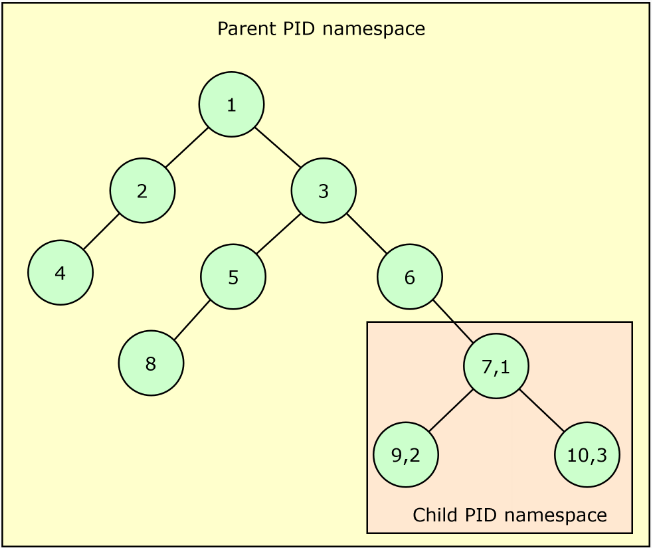
\includegraphics[scale=0.3]{images/processtree.png}
    \caption{An example of nested process with isolation}
    \label{fig:nestedtree}
\end{figure}

\myparagraph{Network Namespaces}
We saw that there are different namespaces for different kind of uses. Let's talk about \textbf{network namespace}. A \textbf{network namespace} allows two processes to perceive a completely different network setup (like routing table, interfaces, firewall, loopback ecc.). Once a network namespace is created we should create additional virtual network interfaces ($veth$) that allows traffic to cross namespace borders and to be delivered to another namespace (fig. \ref{fig:netnamespace}).

An example:
\begin{verbatim}
    sudo ip netns add <netsname> #create a new network namespace named <netsname>
    sudo ip link add veth0-root type veth peer name veth0-ns # Create virtual eth links
    sudo ip link set veth0-ns netns <netsname> #link the namespace to veth0-ns
\end{verbatim}
To interact in the namespace use the command:
\begin{verbatim}
    [sudo] ip netns exec <namespace_name> <command>
\end{verbatim}
After creating namespaces and the virtual "wire" between them and the server in which they are running, we have to assign IP-addresses:
\begin{verbatim}
    sudo ip addr 20.1.1.1/24 dev eth0
    sudo ip netns exec ns1 ip addr add ...
\end{verbatim}
Of course a root namespace is not enough to allow communication with the outside. In fact the server in most cases has a single public IP and multiples private IP. In order to translate private to public IP and forward communication the server needs the NAT.

Other examples of namespaces are:
\begin{itemize}
    \item \textbf{Mount namespaces} that enable the creation of a completely new file system (as a new volume)
    \item \textbf{User namespaces} that allow a process to have root privileges
    \item \textbf{IPC namespaces} that create private inter-process communications
\end{itemize} 

\begin{figure}[H]
    \centering
    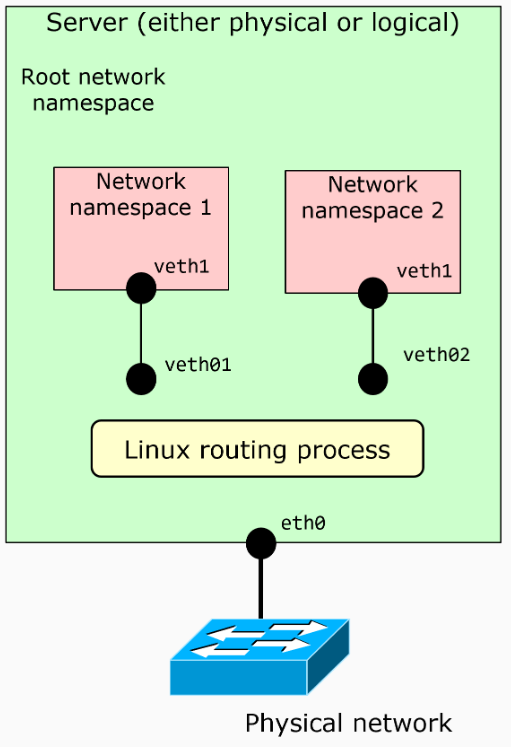
\includegraphics[scale=0.3]{images/netnamespace.png}
    \caption{Schema of a basic network namespace}
    \label{fig:netnamespace}
\end{figure}

\subsubsection{Limitation of these approaches}
Cgroups and Namespaces have some limitations:
\begin{itemize}
    \item beyond process isolation, they can provide a solution for a single server but it takes a lot of command to handle an entire datacenter (composed by hundreds of servers)
    \item they cannot guarantee application portability (such as in the case of VMs). On other computers you'll need to recreate all namespaces from zero
    \item Some commands are not so easy to use
\end{itemize}

\subsubsection{Linux containers}
A solution for cgroups and namespaces problems is \textbf{Linux containers} (LCX). They can provide a lightweight virtualisation (isolation without the complexity of full virtualisation). 
In particular they are an OS-level virtualisation method for running multiple isolated Linux systems on a single control host (the linux kernel is shared across all containers).

The main usage is to run isolate software. LSC allows to configure each container with the list of features it needs by means of a configuration file

Let's see the differences between Containers and Hypervisors in terms of consumes:
\begin{itemize}
    \item containers share the kernel with each other (it can be shared because it's rare that one app need a specific kernel). However the kernel is pretty small compared to libs and bins. So storage requirement is practically the same
    \item containers use less CPU
    \item containers use less memory (RAM)
\end{itemize}

Containers share the same operating system (kernel) as the host. Inside the box they look like a VM (or better a machine), but outside they look like normal processes. They don't emulate hardware and don't run different kernels. Security is not an out-of-the-box feature. Containers are faster and lighter than real VM (they can achieve the same performances of native execution with no virtualisation overhead) but in the other hand VMs provide better isolation, better security and give the possibility to use different OSs.

An overkill feature of the containers is that they are versatile.
\begin{figure}[h!]
    \centering
    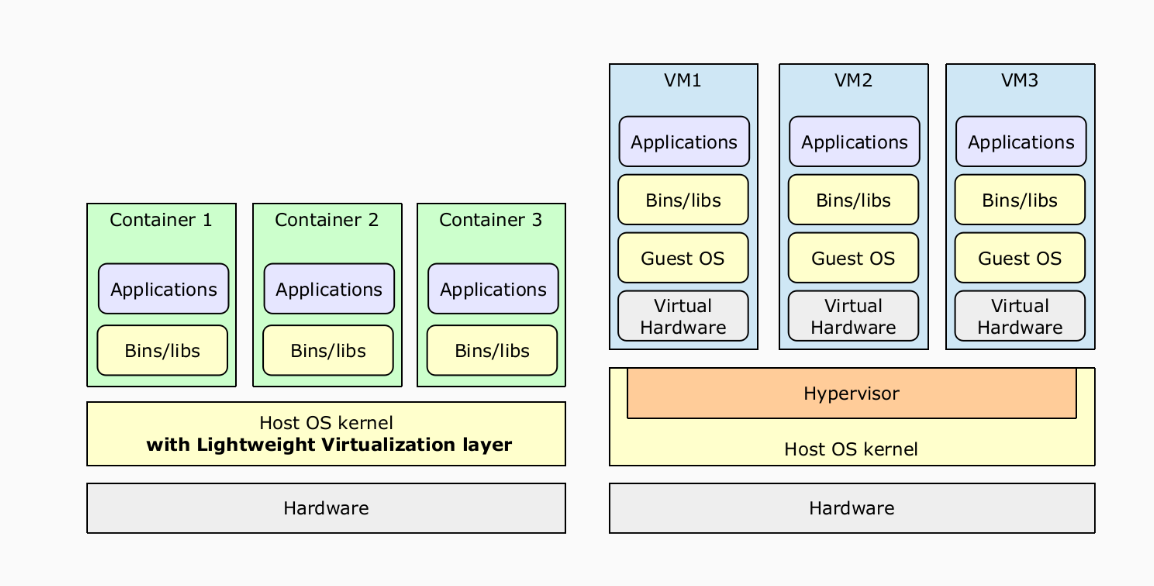
\includegraphics[scale=0.25]{images/contvshyp.png}
    \caption{Containers vs Hypervisors}
    \label{fig:cvs}
\end{figure}

However LXC have some limitations:
\begin{itemize}
    \item A container doesn't memorize the state of a machine. To make possible to migrate containers you should be able to copy and paste the machine state (there are some software tool but not 100\% working). Instead VMs have everything inside, the state too.
    \item There are some resources that you can't isolate completely (like transmission capacity; you can just do some policy)
    \item LCX can't be ported. You always need to create again the container from scratch. This is the most restrictive limitation because it prevent to move servers or stuff running in a container
\end{itemize}

\subsubsection{Docker}
\textbf{Docker} tries to solve the portability problem. It's a service that doesn't focus on virtualisation but directly on applications. Developers up to now had to package applications for each OS (with the possibility to make mistakes or to have other kind of problems); with Docker they can use a light environment (and portable too) that works everywhere they want (locally or in a server).

Docker provides a clean separation between environments and a set of instruction to menage them (it has a simple command line interface to menage containers). Docker containers can run with some TCP ports in order to communicate (Docker itself will create a networking environment that can be shared). However Docker is not a virtualisation engine and doesn't use hardware primitives.

Developers can creates containers and use libraries and dependencies in order to develop their applications. Sometimes they could want to hid code and data from the container (for example if the code is not open-source).

DevOps (who runs the container and uses applications) can login, access, configure and monitor applications that they use.

\myparagraph{Docker Image}
A \textbf{docker image} is a immutable static copy of a container that's not running (like a template). You can push or remove images from a registry. There's a tag that discriminates different versions of images.

\myparagraph{Docker Container}
A \textbf{docker container} is an instance of an image that is running. There could be multiple containers running of the same template.
Container execution can be managed from starting, to stop and restart (containers will maintain changes as long as they're running)

\myparagraph{Docker Registry}
The \textbf{docker registry} is the software repository where images are stored. It can be private or public. Docker provides some commands to manage it pushing or removing images.

When running a container, you can specify some options:
\begin{itemize}
    \item the port where the container is exposed to (the developer can chose and set it)
    \begin{verbatim}
        docker run -p 8080:80 nginx #all the traffic that arrives to the port 8080 will be send to the container whose port is set to 80
    \end{verbatim}
    \item you can run/mount directories that are in the local machine under a certain path tree (so you don't need to build your image with static files inside but dynamically)
    \begin{verbatim}
        docker run -v /html:/usr/share/nginx/html mynginx
    \end{verbatim}
\end{itemize}

Some command to manage containers:
\begin{verbatim}
    docker ps #shows all containers running
    docker ps -a #shows all containers not running but still not closed
    docker run <image> #creates an instance of image on your machine
    docker start <container> #starts the container if stopped.
    docker stop <container> #stops it. Stopped containers don't use resources
    docker kill <container> #kills it
    docker rm <container> #removes it definitely. The state will be lost
    docker exec <container> <command> #executes command on that container.
        #The container must have implemented them
\end{verbatim}

Docker containers are easily reachable from outside. That's because Docker provides a private network, a bridge, IP addresses and configures the NAT and the routing for you. Network operations are carried by the libnetwork component that allow not to use DHCP protocol.
\begin{figure}[h!]
    \centering
    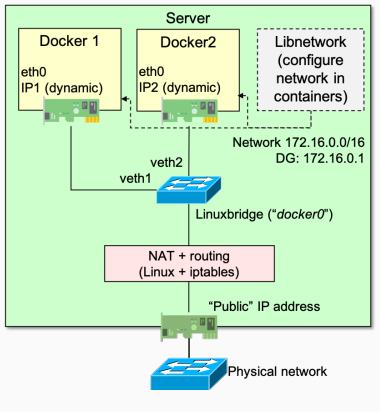
\includegraphics[scale=0.5]{images/docker private network.png}
    \caption{Docker network}
    \label{fig:dckrntwrk}
\end{figure}

\myparagraph{Union file system}
Containers must replicate the file system in order to have their replica. In this way they can guarantee isolation and portability. But how to do that? In fact file systems are quite large and they will require a huge download time and starting a process will become a slow operation. Docker offers a solution:

 The \textbf{Union File System} is a union of merged file systems with a single root. With this technique docker split two layers. a lower layer (read-only) and an upper layer (writable).
If a process wants to modify existing data, OS will copy data just for that process (Copy and Write technique). Simulation is used to hid the entire data and show it with the modifications requested. In this way only differences are stored and you don't need to copy all the bin and libs.

\begin{figure}[h!]
    \centering
    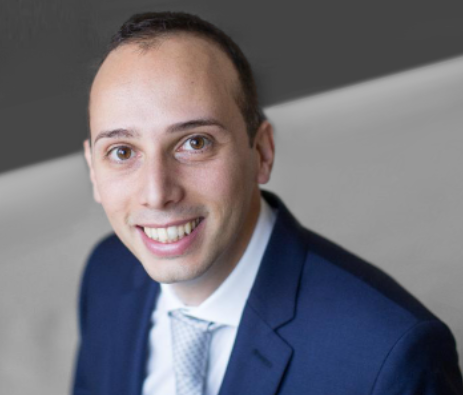
\includegraphics[scale=1.5]{images/king.png}
    \caption{L'unico ed inimitabile Domenico, uno di noi}
    \label{fig:king}
\end{figure}
\clearpage